%% USEFUL LINKS:
%% -------------
%%
%% - UiO LaTeX guides:          https://www.mn.uio.no/ifi/tjenester/it/hjelp/latex/
%% - Mathematics:               https://en.wikibooks.org/wiki/LaTeX/Mathematics
%% - Physics:                   https://ctan.uib.no/macros/latex/contrib/physics/physics.pdf
%% - Basics of Tikz:            https://en.wikibooks.org/wiki/LaTeX/PGF/Tikz
%% - All the colors!            https://en.wikibooks.org/wiki/LaTeX/Colors
%% - How to make tables:        https://en.wikibooks.org/wiki/LaTeX/Tables
%% - Code listing styles:       https://en.wikibooks.org/wiki/LaTeX/Source_Code_Listings
%% - \includegraphics           https://en.wikibooks.org/wiki/LaTeX/Importing_Graphics
%% - Learn more about figures:  https://en.wikibooks.org/wiki/LaTeX/Floats,_Figures_and_Captions
%% - Automagic bibliography:    https://en.wikibooks.org/wiki/LaTeX/Bibliography_Management  (this one is kinda difficult the first time)
%%
%%                              (This document is of class "revtex4-1", the REVTeX Guide explains how the class works)
%%   REVTeX Guide:              http://www.physics.csbsju.edu/370/papers/Journal_Style_Manuals/auguide4-1.pdf
%%
%% COMPILING THE .pdf FILE IN THE LINUX IN THE TERMINAL
%% ----------------------------------------------------
%%
%% [terminal]$ pdflatex report_example.tex
%%
%% Run the command twice, always.
%%
%% When using references, footnotes, etc. you should run the following chain of commands:
%%
%% [terminal]$ pdflatex report_example.tex
%% [terminal]$ bibtex report_example
%% [terminal]$ pdflatex report_example.tex
%% [terminal]$ pdflatex report_example.tex
%%
%% This series of commands can of course be gathered into a single-line command:
%% [terminal]$ pdflatex report_example.tex && bibtex report_example.aux && pdflatex report_example.tex && pdflatex report_example.tex
%%
%% ----------------------------------------------------

\PassOptionsToPackage{square,comma,numbers,sort&compress,super}{natbib}
\documentclass[aps,pra,english,notitlepage,reprint,nofootinbib]{revtex4-1}  % defines the basic parameters of the document
% For preview: skriv i terminal: latexmk -pdf -pvc filnavn
% If you want a single-column, remove "reprint"

% Allows special characters (including æøå)
% \usepackage[mathletters]{ucs}
% \usepackage[utf8x]{inputenc}
% \usepackage[english]{babel}
\usepackage{silence}
\WarningFilter{revtex4-1}{Repair the float}

%% Note that you may need to download some of these packages manually, it depends on your setup.
%% I recommend downloading TeXMaker, because it includes a large library of the most common packages.

\usepackage{physics,amssymb}  % mathematical symbols (physics imports amsmath)
\usepackage{amsmath}
\usepackage{graphicx}
% include graphics such as plots
\usepackage[dvipsnames]{xcolor}           % set colors
% \usepackage{hyperref}         % automagic cross-referencing
%\usepackage{url}
% \usepackage{cleveref}
\usepackage{listings}         % display code
\usepackage{subfigure}        % imports a lot of cool and useful figure commands
\usepackage{subcaption}
%\usepackage{float}
%\usepackage[section]{placeins}
\usepackage{algorithm}
\usepackage[noend]{algpseudocode}
\usepackage{cprotect}
\usepackage{multirow}
\usepackage{array, booktabs}
\newcolumntype{C}[1]{>{\centering\let\newline\\\arraybackslash\hspace{0pt}}m{#1}}
\usepackage[noend]{algpseudocode}
\usepackage{subfigure}
\newcommand{\imp}{\hspace{5pt}\Rightarrow\hspace{5pt}}
\newcommand\numberthis{\addtocounter{equation}{1}\tag{\theequation}}
\usepackage{tikz}
\usepackage{hyperref}         % automagic cross-referencing
\usepackage{cleveref}
\usepackage{comment}
% defines the color of hyperref objects
% Blending two colors:  blue!80!black  =  80% blue and 20% black
\hypersetup{ % this is just my personal choice, feel free to change things
    colorlinks,
    linkcolor={red!50!black},
    citecolor={blue!50!black},
    urlcolor={blue!80!black},
breaklinks=true}
\urlstyle{same}

\renewcommand{\bibsection}{\section*{References}}
\newcommand{\psp}{\hspace{1pt}}
% ===========================================

\begin{document}

\title{\texorpdfstring{
        \begin{Large}Project 2
\end{Large}\\\vspace{5pt}FYS-STK4155}{Lg}}
\author{Erik Joshua Røset \& Oskar Idland}
\date{\today}
\affiliation{University of Oslo, Department of Physics}

\begin{abstract}
    \centering
    In this project, we extend our exploration of machine learning techniques to include advanced optimization algorithms and neural networks. We implement and analyze gradient descent methods, including Stochastic Gradient Descent (SGD), as well as feed-forward neural networks. Our analysis focuses on the mathematical foundations of backpropagation, activation functions, and regularization techniques. We apply these methods to both regression and classification tasks, using synthetic data generated through the Franke function and the Wisconsin Breast Cancer dataset. By comparing our implementations with established libraries like Scikit-learn and PyTorch, we gain insights into the practical considerations of neural network development and optimization. Our results demonstrate the importance of activation functions, initialization strategies, and regularization methods in training effective neural networks. We also highlight the impact of optimization techniques on model convergence and generalization, providing a comprehensive overview of the fundamental building blocks of modern machine learning systems.

    % We have explored various regression techniques and resampling methods within the context of machine learning, motivated by the need to develop robust models that can accurately predict and generalize from complex datasets. The main objective was to analyze and compare the performance of Ordinary Least Squares (OLS), Ridge, and Lasso regression in fitting synthetic and real-world data, focusing on the bias-variance tradeoff and model generalizability. We applied these regression techniques to the Franke function, a synthetic benchmark used in numerical analysis, and extended our analysis to cosmological N-body simulation data generated using the public G\begin{scriptsize}ASOLINE\end{scriptsize}2 SPH code. To assess model performance and generalization, we employed resampling methods such as bootstrap and $k$-fold cross-validation, examining how they help to evaluate model accuracy under different training and test data conditions. Due to runtime limitations we only tested polynomial degrees up to 31 for the cosmological data, and found that the model was insufficient in representing its intricate structure. As a result, introducing regularization with the Ridge and Lasso techniques led to poor model performance, while the employment of resampling methods proved to show negligible improvements. For future studies, optimizing our code and testing larger polynomial degrees could be an area of interest.
\end{abstract}
\maketitle
\onecolumngrid
\begin{center}
    \vspace{-15pt}
    % LINK TO REPOSITORY
    \href{https://github.com/Oskar-Idland/FYS-STK4155-Projects}{https://github.com/Oskar-Idland/FYS-STK4155-Projects}%{GitHub Repository}
    \vspace{5pt}
\end{center}
\twocolumngrid
% ===========================================

%#TODO punctuate the equations

\section{Introduction}\label{sec:introduction}
\begin{comment}
  #TODO: Maybe angle it more towards exploring breast cancer?
  #TODO: Mention the appendix and what it contains
\end{comment}
% The rapid advancement of artificial intelligence (AI) and machine learning has significantly impacted various fields, with medical imaging and diagnostics being among the most benefited areas \cite{litjens2017survey}. A key development in this field is the use of Convolutional Neural Networks (CNNs), a type of deep learning model known for being effective in image recognition and classification. CNNs are widely used in healthcare, especially for important tasks like tumor detection and disease classification, where accuracy and efficiency are crucial \cite{9395920}. However, many traditional neural networks, including CNNs, need a lot of computational power, which can make them less suitable for use in resource-limited environments \cite{howard2017mobilenetsefficientconvolutionalneural}. 

To address this, more efficient architectures like MobileNet and ResNet have been created. MobileNet is designed to be lightweight and efficient, making it ideal for tasks like medical image classification \cite{howard2017mobilenetsefficientconvolutionalneural}. ResNet, on the other hand, uses residual connections to help train deep networks, which solves the degradation problem and improves performance in complex image recognition tasks \cite{he2015deepresiduallearningimage}. Together, these architectures offer a range of solutions for efficient and effective deep learning in medical imaging applications.

This study aims to evaluate and compare the performance of various neural network architectures on a breast cancer histopathological dataset, focusing on three specific models: a custom CNN, MobileNet, and ResNet101. These models are selected based on their differing complexities, training requirements, and computational efficiencies. In this analysis, we will compare how well these models handle a small and imbalanced dataset, aiming to understand how different architectures affect classification accuracy and performance in medical applications.

This report is organized as follows: First, we introduce the theoretical concepts behind neural networks, CNNs, MobileNet, and ResNet, along with the relevant evaluation metrics. Next, we discuss the methods and implementation, including data preprocessing and model architectures. We then present the results, comparing the performance of the models. Finally, we conclude by summarizing our findings and identifying the most suitable model for handling complex data.

% In \cref{sec:theory} we present relevant background theory, the majority of which has been sourced from the lecture notes by Morten Hjorth-Jensen \cite{notes}. We go into detail explaining central concepts such as OLS, Ridge and Lasso regression, the bias-variance tradeoff and two crucial resampling methods; bootstrapping and cross-validation, both of which will be implemented in this work. A few of the most important expressions introduced in this section are derived in \cref{appsec:derivations}. Our methodology is explained in \cref{sec:methods}, specifically how we define the essential design matrix, scale our data and implement the regression and resampling techniques. We also give an overview of our code structure and present the cosmological simulation data. In \cref{sec:results discussion} we present, interpret and discuss the results of our analyses in light of expectations based on our previous knowledge of the implemented regression and resampling methods. In \cref{appsec:figures} we include some additional figures that are not essential to our discussions, yet still referred to in the aforementioned section because they are necessary in reasoning our choice of presented results. Lastly, we summarize and conclude the main findings of our work in \cref{sec:conclusion}, and provide some open questions for further exploration.

% ===========================================
\section{Theory}\label{sec:theory}

% 
\section{Neural networks}

Neural Networks are computational models inspired by biological neural networks in the human brain. They learn by example, rather than being explicitly programmed with detailed instructions for a task. This learning process uses data split into training and testing sets. 

A neural network consists of layers of interconnected units called neurons. Each neuron receives multiple inputs, combines them using adjustable factors called weights, applies a mathematical function to decide its output, and then passes this output to the next layer. The weights determine the strength of the connections between neurons, and by fine-tuning these weights, the network learns to identify patterns and improve its performance.

Mathematically, this process can be represented as in Equation \ref{neuralnetwork}.

\begin{equation}
   y = f\left(\sum_{i=1}^{n} w_i x_i\right) = f(z)
   \label{neuralnetwork}
\end{equation}

where \( y \) is the output, \( w_i \) are the weights, \( x_i \) are the input values, and \( f(z) \) is the activation function applied to the combined inputs.

\subsection{Convolution Neural Network}


There are various types of neural networks designed for specific tasks, and among them, Convolution Neural Networks (CNN) are one of the most widely used and impactfull. CNN were originally created for tasks like recognizing handwritten characters. Today, they are more central to many advancements in artificial intelligence, particularly in image processing and computer vision. CNNs are similar to traditional Neural Networks in that they consist of neurons with adjustable weights that learn patterns from data.

%Through training methods like backpropagation and gradient descent, CNNs improve their accuracy by adjusting these weights over time. 

%What makes CNNs unique is their ability to leverage the specific properties of images, such as identifying edges, textures, and shapes, while requiring fewer parameters than traditional neural networks. This efficiency makes CNNs faster, more scalable, and ideal for tasks like object detection, face recognition, and autonomous vehicle navigation.


CNNs are great at using the natural structure of visual data. Unlike other types of data, images have unique features like edges, textures, and shapes. CNNs are specifically designed to recognize and process these features efficiently, requiring less parameters than the traditional neural networks. This efficiency makes CNNs faster and easier to use on large tasks, and very effective for things like object detection and face recognition. They are specifically built for image data, with a structure that aligns with the way images are organized. Unlike traditional neural networks, CNN layers arrange neurons in three dimensions: width, height, and depth.

To understand why CNNs are so effective, it's important to first examine how neural networks process data. Neural networks commonly use an affine transformation, a method that works for any type of data that can be flattened into a single list of numbers. However, for structured data like images, this approach has a significant drawback: it ignores the natural structure of the data. Images are multi-dimensional grids of pixels where the spatial arrangement, such as width, height and depth is crucial. Flattening these grids into a single vector removes this valuable information. This is where convolutions layers is essential.

\subsubsection{ Convolution layers}

CNNs are able to recognize patterns in images because of their convolution layers. Convolution layers are a type of hidden layer in CNNs. Each convolution layer takes an input, applies a transformation to it, and passes the transformed data to the next layer. This transformation is performed through the convolution.
Convolution a mathematical operation that processes structured data while maintaining its original form and relationships. It applies a filter (or kernel) to the input data, combining nearby values to extract features such as edges or textures in images. Mathematically, convolution is represented as:

\begin{equation}
    y(t) = \int x(a)w(t-a) \, da
\end{equation}

where \( x(a) \) represents the input,  \( w(t-a) \) is the filter or kernel, which slides over the input to process it locally and \( y(t) \)is the output after applying the convolution.

For digital data like images, this integral is replaced by a summation in the discrete form as in Equation \ref{conv_dis}

\begin{equation}
    y(t) = \sum_{a=-\infty}^{\infty} x(a)w(t-a)
\label{conv_dis}
\end{equation}

This operation ensures that the structure of the data is maintained, making it particularly suited for tasks involving visual data. Convolution Neural Networks use this property by arranging neurons in width, height, and depth to efficiently process and learn from structured data.














\subsubsection{MobileNet}

MobileNet is a lightweight and efficient deep neural network architecture designed specifically for mobile and embedded vision tasks \cite{howard2017mobilenetsefficientconvolutionalneural}. It reduces computational complexity and memory usage by employing depthwise separable convolutions instead of traditional convolutions \cite{howard2017mobilenetsefficientconvolutionalneural}. This involves splitting the standard convolution process into two distinct steps: a depthwise convolution, which applies a single filter to each input channel, and a pointwise convolution (1×1 convolution), which combines the outputs to form new features \cite{howard2017mobilenetsefficientconvolutionalneural}. This factorization drastically reduces the computational cost and model size, making MobileNet an ideal choice for resource-constrained devices \cite{howard2017mobilenetsefficientconvolutionalneural}.

The depthwise convolution operation in MobileNets can be mathematically represented as follows:

\[ G_{k,l,m} = \sum_{i,j} K_{i,j,m} \cdot F_{k+i-1,l+j-1,m} \]

\begin{itemize}
    \item  \( G_{k,l,m} \): Output feature map at position \( (k, l) \) for the \( m \)-th channel \cite{howard2017mobilenetsefficientconvolutionalneural}.
    \item  \( K_{i,j,m} \): Depthwise convolution kernel for the \( m \)-th channel, of size \( D_K \times D_K \) \cite{howard2017mobilenetsefficientconvolutionalneural}.
    \item  \( F_{k+i-1,l+j-1,m} \): Input feature map at the shifted position \( (k+i-1, l+j-1) \) for the \( m \)-th channel \cite{howard2017mobilenetsefficientconvolutionalneural}.
    \item \( i, j \): Kernel index variables, ranging over the kernel size \( D_K \) \cite{howard2017mobilenetsefficientconvolutionalneural}.
\end{itemize}

This formula indicates that for each output position \( (k, l) \) and each channel \( m \), the convolution is computed by applying a kernel \( K_{i,j,m} \) to the corresponding input positions \( (k+i-1, l+j-1) \) \cite{howard2017mobilenetsefficientconvolutionalneural}. The kernel filters the input feature map \( F \) for each channel independently, without mixing features between channels \cite{howard2017mobilenetsefficientconvolutionalneural}. This selective filtering significantly reduces the computational resources required as compared to traditional convolutions that combine inputs across all channels \cite{howard2017mobilenetsefficientconvolutionalneural}.





\subsection{Residual Networks (ResNet)}
Deep neural networks often face two significant challenges: the \textit{degradation problem} and the \textit{vanishing/exploding gradients problem} \cite{he2015deepresiduallearningimage}. As networks increase in depth, their performance tends to saturate, and adding more layers can lead to higher training errors, a phenomenon known as the degradation problem. Additionally, during backpropagation, gradients can become extremely small (vanishing) or excessively large (exploding), which hampers the effective training of very deep networks \cite{he2015deepresiduallearningimage}.

To address these challenges, Residual Networks (ResNet) introduce a \textit{residual learning framework}. Instead of learning the full mapping \( H(x) \) from inputs to outputs, ResNet learns the \textit{residual mapping}, \( F(x) = H(x) - x \). This reformulation allows the model to compute the output as \( H(x) = F(x) + x \), where \( x \) is the input. The residual learning approach makes it easier for the network to optimize, as the residual function \( F(x) \) often has a simpler structure than the direct mapping \( H(x) \) \cite{he2015deepresiduallearningimage}.

At the core of ResNet is the \textit{residual block} \cite{he2015deepresiduallearningimage}, which includes a \textit{skip connection (shortcut)} that bypasses one or more layers \cite{he2015deepresiduallearningimage}. These skip connections add the input \( x \) directly to the output of the block, facilitating the flow of gradients during backpropagation \cite{he2015deepresiduallearningimage}. This design mitigates the vanishing gradient problem and allows the network to retain information from earlier layers, making it possible to train networks with much greater depth \cite{he2015deepresiduallearningimage}.

ResNet architectures are built by stacking multiple residual blocks, enabling the construction of very deep networks. Popular versions include:
\begin{itemize}
    \item \textbf{ResNet-50:} A network with 50 layers \cite{he2015deepresiduallearningimage}.
    \item \textbf{ResNet-101:} A deeper network with 101 layers \cite{he2015deepresiduallearningimage}.
    \item \textbf{ResNet-152:} An even deeper variant with 152 layers \cite{he2015deepresiduallearningimage}.
\end{itemize}
These networks typically start with an initial convolutional layer, followed by multiple residual blocks grouped into stages, and conclude with a fully connected layer for classification tasks.

ResNet achieves state-of-the-art performance in tasks like image classification, particularly in the ImageNet Large Scale Visual Recognition Challenge (ILSVRC) \cite{he2015deepresiduallearningimage}. For example, ResNet achieved a top-5 error rate of 3.57\% on ImageNet \cite{he2015deepresiduallearningimage}. The introduction of residual learning and skip connections enables the training of networks with hundreds or even thousands of layers, solving critical challenges in deep learning and setting a new standard for neural network design \cite{he2015deepresiduallearningimage}.


Before the final fully connected layer, ResNet employs \textit{Global Average Pooling (GAP)} to reduce each feature map into a single value \cite{he2015deepresiduallearningimage}. This technique provides a compact representation of the feature maps, improving computational efficiency and reducing the risk of overfitting.



\section*{Evaluation Metrics}
\subsection*{Precision}
\textbf{Formula:}
\[
\text{Precision} = \frac{\text{True Positives (TP)}}{\text{True Positives (TP)} + \text{False Positives (FP)}}
\]

Precision measures the proportion of true positive predictions among all instances predicted as positive. This metric is particularly important in scenarios where false positives carry significant costs, such as in fraud detection or medical testing. A high precision indicates that the model has effectively minimized false positive predictions \cite{hossin2015review}.

\subsection*{Recall (Sensitivity or True Positive Rate)}
\textbf{Formula:}
\[
\text{Recall} = \frac{\text{True Positives (TP)}}{\text{True Positives (TP)} + \text{False Negatives (FN)}}
\]

 
Recall quantifies the ability of the model to identify actual positive cases. It is critical in applications where missing positive cases (false negatives) have severe implications, such as in medical diagnoses or safety-critical systems \cite{hossin2015review}.

\subsection*{F1-Score}
\textbf{Formula:}
\[
\text{F1-Score} = 2 \times \frac{\text{Precision} \times \text{Recall}}{\text{Precision} + \text{Recall}}
\]


The F1-score provides a harmonic mean of Precision and Recall, offering a balanced evaluation metric that is particularly useful in datasets with imbalanced class distributions. It penalizes extreme differences between Precision and Recall, ensuring a more holistic assessment of model performance \cite{hossin2015review}.

\subsection*{Accuracy}
\textbf{Formula:}
\[
\text{Accuracy} = \frac{\text{True Positives (TP)} + \text{True Negatives (TN)}}{\text{Total Instances}}
\]


Accuracy measures the overall proportion of correctly classified instances among all predictions. While it is easy to compute and interpret, it can be misleading in imbalanced datasets where one class dominates, necessitating supplementary metrics like F1-score \cite{hossin2015review, dalianis2018clinical}.

\subsection*{Confusion Matrix}
These metrics are derived from the confusion matrix, which provides a detailed breakdown of model predictions:
\begin{itemize}
    \item \textbf{True Positives (TP):} Correctly predicted positive instances.
    \item \textbf{True Negatives (TN):} Correctly predicted negative instances.
    \item \textbf{False Positives (FP):} Negative instances incorrectly predicted as positive.
    \item \textbf{False Negatives (FN):} Positive instances incorrectly predicted as negative.
\end{itemize}

The confusion matrix serves as the foundation for most classification metrics, offering insights into both model strengths and weaknesses \cite{hossin2015review, dalianis2018clinical}.




%### Notes:

%- Replace `hossin2015review` and `dalianis2018clinical` with the appropriate citation keys from your `.bib` file.
%- Make sure your `.bib` file includes the sources:
%  - Hossin, M. (2015). *A Review on Evaluation Metrics for Data Classification Evaluations*.
 % - Dalianis, H. (2018). *Clinical Text Mining: Secondary Use of Electronic Patient Records*.


\section{Methods \& Implementation}\label{sec:methods}

% 
\subsection{Regression Analysis}
To explore the optimization methods discussed in the theory \cref{sec:theory}, we first consider a regression problem using the Franke function. This function is a widely used benchmark for regression tasks, as it provides a smooth, non-linear surface that can be sampled to generate noisy data. We generate a dataset by sampling the Franke function with added Gaussian noise, which we then use to train and evaluate our regression models. We fit our model to this data with a polynomial design matrix, after splitting it into training and test sets, and evaluate the model's performance using metrics like the mean squared error (MSE) and \( R^2 \) score.

Regression models have many parameters, making it impossible (or at least impractical) to iterate over all possible combinations. We use grid search to explore two parameters at a time. We then zoom in on the most promising regions to find the optimal parameters. After finding a suitable set of parameters, we continue the search for the next set of parameters.

\subsubsection{Plain Gradient Descent}
\paragraph*{No Momentum:}
To be sure we understand the basic principles of gradient descent, we start by implementing a simple gradient descent algorithm for linear regression. We use the MSE as our cost function and compute the gradient of the cost function with respect to the model parameters. We then update the parameters using the gradient and iterating over a set of learning rates.
\paragraph*{Momentum:}
We then extend our implementation to include momentum. Now we iterate over all possible values of the momentum and learning rate to find the optimal combination for our model. After creating a general overview of the entire parameter space, we zoom in on the most promising regions to find the optimal parameters. This process will be repeated for the other optimization methods as well.

\subsubsection{Stochastic Gradient Descent}
\paragraph*{No Momentum:}
Continuing with stochastic gradient descent, we implement a simple version of the algorithm and apply it to our regression problem. We then begin by iterating over all possible learning rates and batch sizes to find the optimal combination. We then zoom in on the most promising regions to find the optimal parameters.
\paragraph*{Momentum:}
Secondly, we use the ideal learning rate, and then iterate over possible values of the momentum to find the optimal combination. We then zoom in on the most promising regions to find the optimal parameters.

Moving on to the more advanced optimization methods, we implement AdaGrad, RMSprop, and Adam. We follow the same procedure as before, iterating over all possible learning rates and momentum values to find the optimal combination. We note the optimal values to use in the neural network implementation.

\begin{comment}
  #TODO: Update if we iterate over momentum and rho values as well
\end{comment}

\subsubsection{AdaGrad}
\paragraph{No Momentum:}
For both the regular and stochastic versions of AdaGrad, we iterate over all possible learning rates to find the optimal value.

\paragraph{Momentum:}
Using the optimal values found in the previous step, we then iterate over all possible values of the momentum to find the optimal value to pair with the learning rate.

\subsubsection{RMSprop \& Adam}
\paragraph{No Momentum:}

\subsection{Neural Networks}
In order to explore the optimization methods discussed in the theory section, we consider again a regression problem on the Franke function, and also a classification problem on the Wisconsin Breast Cancer dataset. % #TODO cite sklearn
The hyperparameter space is vast, and in order to effectively produce results we narrow down the possibilities by first deciding on a singular network model to base our work on. This entails initializing our models with pseudo-random weights sampled from a univariate normal distribution with zero mean and a variance of one. The same goes for the biases, but with an added constant of 0.01 in order to break symmetry. With the focus on exploring the influence of hyperparameters, we choose to keep the network architecture simple, with a single hidden layer and a fixed number of nodes. This allows us to focus on the effects of the learning rate, batch size, and regularization strength on the network's performance.
\subsubsection{Franke Function Regression}

We first validated our neural network implementation using the Franke function regression problem. Input data was generated by sampling the Franke function on a uniform grid of \( 100 \times 100 \) points over the unit square \( [0,1]\times[0,1] \). To simulate measurement noise, we added Gaussian noise with mean zero and standard deviation \( \sigma = 0.01 \) to the function values.

The input coordinates \( (x,y) \) were used to generate a design matrix with polynomial features up to degree 4, chosen to match the complexity of the Franke function's structure. The dataset was split into training \( (80\%) \) and test \( (20\%) \) sets using scikit-learn's \verb|train_test_split function|. Both input features and target values were standardized using StandardScaler, with the scaling parameters computed only from the training set to prevent data leakage.

The network was configured with a single hidden layer of 15 nodes, empirically chosen as a balance between model complexity and computational efficiency. The output layer consisted of a single node for regression. We initialized weights from a normal distribution \( \mathcal{N} (0,1) \) and biases with a small constant offset of 0.01 to break symmetry in the network's initial state.

For our systematic hyperparameter exploration, we established a standard configuration:
\begin{itemize}
    \item Activation function: Sigmoid in the hidden layer
    \item Cost function: Mean Squared Error (MSE)
    \item Optimizer: AdaGrad with momentum (\( \eta \) = 0.01, \( \gamma \) = 0.8)
    \item Regularization rate: \( \lambda \) = 0.0001
\end{itemize}

These baseline parameters were chosen based on preliminary experiments showing stable convergence without excessive overfitting. This configuration served as our control point, allowing us to systematically vary individual parameters while holding others constant.

\paragraph*{Epochs vs batch size:}
Our first step was to explore the relationship between the number of epochs and the batch size. We iterated over epoch sizes \( (100, 500, 1000, 2000) \) and number of batches \( (1, 10, 20, 50, 100) \) and calculated the score metrics for each combination. From here we went further with using 500 epochs and 20 batches for the rest of the analysis.

\paragraph*{Learning rate (\( \eta \)) vs Regularization (\( \lambda \)):}
This was conducted in similar fashion to the previous step, with the learning rate \( \eta \) ranging from values (\( 1e^{-4} \) to \( 1e^{-1} \) and 0.5), and the regularization parameter \( \lambda \) ranging from (\( 1e^{-5} \) to \( 1e^{-1} \)).

\paragraph*{Schedulers:}\label{subsec:nn_schedulers}
To compare the different learning rate schedulers discussed in \cref{sec:learning_rate_tuning}, we implemented one instance of each of them with the standard learning rate. For plain momentum and Adagrad with momentum, we used the parameters \( \gamma = 0.8 \) again. For Adam, we used the parameters \( \rho = 0.9, \rho_2 = 0.999 \). RMPprop had the same \( \rho \) value as Adam. To ensure numerical stability, we used a small value of \( \epsilon = 1e^{-8} \) for all the optimizers. The momentum and decay parameters were chosen based on common values in deep learning literature that typically show good performance across different problems. % #TODO cite

Training progression was monitored by computing both MSE and \( R^2 \) scores on the training data at each epoch. Convergence was defined quantitatively as the point where the relative difference between the mean MSE of the last 10 epochs and the current MSE fell below \( 10^{-2} \), providing a relative convergence criterion for comparing optimizer efficiency. For final model evaluation, we computed these metrics on the held-out test set to assess generalization performance.
\subsubsection{Breast Cancer Classification}

For the classification task, we used the Wisconsin Breast Cancer dataset, which contains 30 features computed from digitized images of fine needle aspirates (FNA) of breast mass, with binary labels indicating malignant or benign tumors. The data was split into training and test sets using an 80-20 split. Unlike the Franke function data, only the input features were standardized since the target values are binary.

We maintained the same basic network architecture as in the regression task, initially using a single hidden layer with 15 nodes. The sigmoid activation function was employed in both the hidden and output layers, with the output layer producing a single value representing the probability of malignancy. For this binary classification problem, we used the logistic regression cost function \cref{logistic_cost}.

Given the relatively small size of the dataset compared to the Franke function case, we reduced the training duration to 20 epochs with 20 batches. The initial configuration used a regularization parameter \( \lambda \) = 0.01 and the Adam optimizer with learning rate \( \eta \) = 0.001, and momentum parameters \( \rho \) = 0.9, \( \rho_2 \) = 0.999. Model performance was evaluated using both training and test set accuracy scores.

Our investigation proceeded in three main stages:

\paragraph*{Learning Rate and Regularization Parameter:}
Learning Rate and Regularization: We performed a grid search over learning rates and regularization parameters, both ranging from \( 10^{-5} \) to \( 10^{-1} \). This explored the balance between model convergence speed and stability versus overfitting prevention.

\paragraph*{Network Architecture:}
We systematically investigated the effect of network depth and width by varying:
\begin{itemize}
    \item Number of hidden layers: 1 to 3 layers
    \item Neurons per layer: 5 to 25 neurons, in steps of 5
\end{itemize}
Each configuration was trained with the previously determined optimal learning rate and regularization parameter to isolate the effect of architecture changes.

\paragraph*{Activation Functions:}
Maintaining the 15-neuron architecture, we compared three different activation functions in the hidden layers:
\begin{itemize}
    \item Sigmoid
    \item ReLU
    \item Leaky ReLU
\end{itemize}
This comparison was performed across networks with 1 to 3 hidden layers to understand how different activation functions affect the network's learning capacity at varying depths. The output layer retained the sigmoid activation function to maintain proper probability outputs for classification.

\subsection{Logistic Regression}
To evaluate different approaches to classification of the Wisconsin Breast Cancer dataset, we implemented logistic regression alongside our neural network. While our neural network used a single hidden layer, logistic regression represents an even simpler model that can be viewed as a neural network without any hidden layers, using only a sigmoid activation function on the output.

Using the same preprocessed dataset as in our neural network analysis (standardized features, 80-20 train-test split), we implemented logistic regression with the standard sigmoid function and logistic regression cost function.

To enable direct comparison with our neural network results, we performed a similar grid search over:

\begin{itemize}
    \item Learning rates \( \eta \): [\( 10^-{5,} 10^{-4}, 10{^-}3, 10^{-2}, 10^{-1} \)]
    \item Regularization \( \lambda \): [\( 10^{-5}, 10^{-4}, 10^{-3}, 10^{-2}, 10^{-1} \)]
\end{itemize}
We maintained consistency with our other implementations by using stochastic gradient descent with batch size 20 and 20 epochs. The model's performance was evaluated using the accuracy score on both training and test sets, allowing comparison between the simpler logistic regression and the single-hidden-layer neural network approach.

\subsection{Benchmark Implementations}
For validation and comparison purposes, we implemented equivalent models using established machine learning frameworks - PyTorch\cite{PyTorch} and scikit-learn\cite{scikit-learn}. This allowed us to benchmark our implementations against industry-standard tools.

For the Franke function regression problem, we created a PyTorch neural network with a similar architecture to our implementation: an input layer of 2 neurons (for x and y coordinates), two hidden layers of 50 and 25 neurons with sigmoid activation functions, and a single output neuron with linear activation. The model was trained using stochastic gradient descent with a batch size of 32 over 2000 epochs.

For the breast cancer classification task, we implemented both a PyTorch neural network and scikit-learn's LogisticRegression. The PyTorch model consisted of two hidden layers (10 and 5 neurons) with sigmoid activations, followed by a binary output layer. For direct comparison with our logistic regression implementation, we utilized scikit-learn's implementation with L2 regularization and the LBFGS optimizer. Both frameworks' models were trained on the same standardized data splits as our implementations to ensure fair comparison.

To maintain consistency in evaluation metrics, we used the same performance measures (MSE and $R^2$ for regression, accuracy for classification) across all implementations. This provided a robust framework for validating our custom implementations against established tools.

\subsection{Program}\label{sec:program}
\subsubsection{Code Structure}\label{subsec:codestructure}
All the source code that we developed and used to produce our results is available on our GitHub repository, linked in \cref{appsec:code} in \verb|Project_2/src|. The \verb|README.md| file contains the entire project file structure. To replicate our exact results, use the provided \verb|requirements.txt| file to install the necessary packages. Our code is divided into the following files and notebooks.

\paragraph*{Regression Analysis}
\verb|RegressionModel.py| contains the classes for the regression models.

\verb|regression_anal.ipynb| contains the analysis of the Franke function data, which we used to validate our implementation.

\paragraph*{Neural Networks}
\verb|FFNN.py| contains the classes for the neural networks.

\verb|nn_Franke.ipynb| contains the analysis of the Franke function to validate the implementation of neural networks.

\verb|nn_breast_cancer.ipynb| contains the analysis of the breast cancer data using neural networks. This is where we truly optimize the hyperparameters of the neural networks.

\verb|logistic_regression_anal.ipynb| contains the analysis of the breast cancer data using logistic regression.

\verb|nn_pytorch.ipynb| Contains the analysis of the Franke function and the Wisconsin Breast Cancer dataset using PyTorch and the analysis of the latter dataset using scikit-learn's logistic regression implementation.

\verb|activation_funcs.py| contains the activation functions used in the neural networks.

\verb|cost_funcs.py| contains the cost functions used in the neural networks.

\paragraph*{Miscellaneous}
\verb|utils.py| contains utility functions used throughout the project. This includes plotting, data generation and other repetitive tasks.

\subsection{Tools}\label{subsec:tools}

All our code is written in Python (3.12) \cite{Python},  and we used scikit-learn \cite{scikit-learn} and PyTorch\cite{PyTorch} to test against our models. To vectorize our code we used \verb|numpy| \cite{Numpy}, and for visualization we used \verb|matplotlib.pyplot| \cite{Matplotlib}. All python packages and their versions can be found in our \verb|requirements.txt|. Code completion and debugging was done in Visual Studio Code \cite{VSCode} with additional assistance of GitHub Copilot \cite{Copilot}. We used \verb|git| \cite{Git} for version control, and \verb|GitHub| \cite{GitHub} for remote storage of our code.


\section{Results \& Discussion}\label{sec:results discussion}
\subsection{Regression Analysis}
\subsubsection{Plain and Stochastic Gradient Descent}
\begin{figure}[h!]
    \centering
    \includegraphics[width = .4\textwidth]{../figs/a_2_parameter_overview.pdf}
    \caption{Overview of the entire parameter space, plotting learning rate against momentum,  using plain gradient descent. The optimal parameters are marked with a red cross, to use as a starting point for further analysis.}
    \label{fig: param_overview}
\end{figure}

\begin{figure}[h!]
    \centering
    \includegraphics[width = .4\textwidth]{../figs/GD_eta_gamma.pdf}
    \caption{Narrowed down parameter space from \cref{fig: param_overview}.}
    \label{fig: param_narrowed}
\end{figure}

\begin{figure}[ht!]
    \centering
    \includegraphics[width = .4\textwidth]{../figs/SGD_batch_eta_.pdf}
    \caption{Plotting batch size, against learning rate, using stochastic gradient descent.}
    \label{fig: SGD_batch_eta}
\end{figure}

\begin{figure}[ht!]
    \centering
    \includegraphics[width = 0.4\textwidth]{../figs/SGD_batch_gamma.pdf}
    \caption{Plotting the batch size against the momentum, using stochastic gradient descent. Using a learning rate of $0.2$}
    \label{fig: SGD_batch_gamma}
\end{figure}

\subsubsection{AdaGrad}
\begin{figure}[ht!]
    \centering
    \includegraphics[width = 0.4\textwidth]{../figs/AdagradMomentum_eta_gamma.pdf}
    \caption{Plotting the learning rate against the momentum, using regular AdaGrad}
    \label{fig: AdagradMomentum_eta_gamma}
\end{figure}

\begin{figure}[ht!]
    \centering
    \includegraphics[width = 0.4\textwidth]{../figs/AdagradMomentum_stochastic_eta_gamma.pdf}
    \caption{Plotting the learning rate against the momentum, using stochastic AdaGrad. The batch size is set to 20.}
    \label{fig: AdagradMomentum_stochastic_eta_gamma}
\end{figure}

\subsubsection{RMSprop}
\begin{figure}[ht!]
    \centering
    \includegraphics[width = 0.4\textwidth]{../figs/RMS_Prop_eta_rho.pdf}
    \caption{Plotting the learning rate against the decay rate, using RMSprop}
    \label{fig: RMS_Prop_eta_rho}
\end{figure}

\begin{figure}[ht!]
    \centering
    \includegraphics[width = 0.4\textwidth]{../figs/RMS_Prop_stochastic_eta_rho.pdf}
    \caption{Plotting the learning rate against the decay rate, using stochastic RMSprop. The batch size is set to 20.}
    \label{fig: RMS_Prop_stochastic_eta_rho}
\end{figure}

\subsubsection{Adam}
\begin{figure}[ht!]
    \centering
    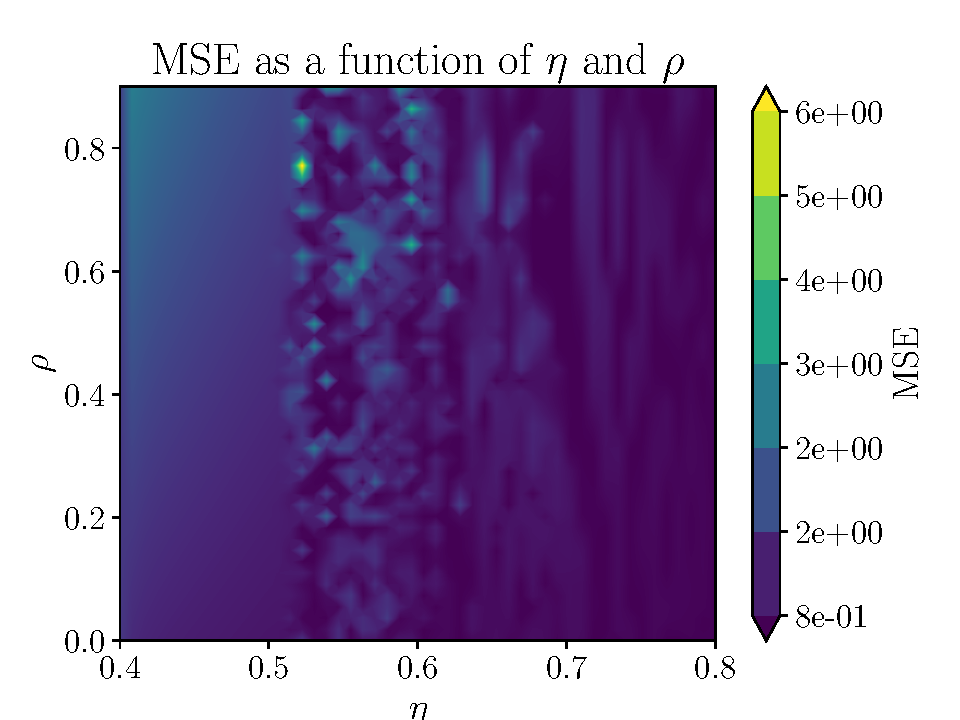
\includegraphics[width = 0.4\textwidth]{../figs/Adam_eta_rho.pdf}
    \caption{Plotting the learning rate against the decay rate. We have set the same value for $\rho_1$ and $\rho_2$, using Adam}
    \label{fig: Adam_eta_rho.pdf}
\end{figure}

\begin{figure}[ht!]
    \centering
    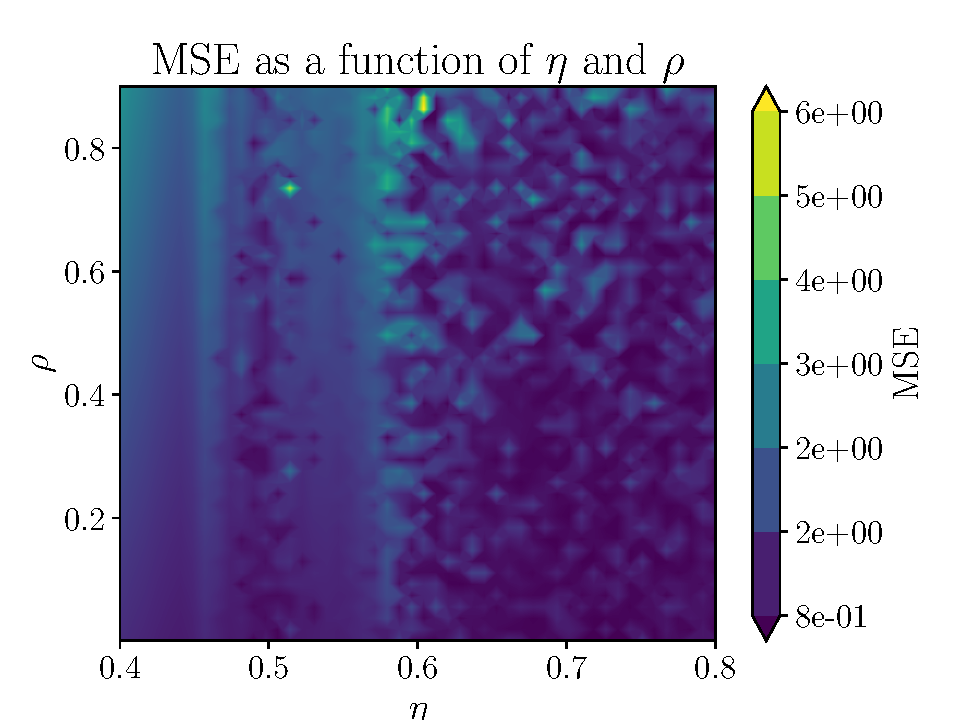
\includegraphics[width = 0.4\textwidth]{../figs/Adam_stochastic_eta_rho.pdf}
    \caption{Plotting the learning rate against the decay rate, using stochastic Adam. The batch size is set to 20, and the same value for $\rho_1$ and $\rho_2$ is used.}
    \label{fig: Adam_stochastic_eta_rho.pdf}
\end{figure}
  
Look at \cref{fig: param_overview} and \cref{fig: param_narrowed} we see a clear interval of parameters which gave low MSE values. Using the best parameters found as a starting point, we continued searching \cref{fig: SGD_batch_eta} and \cref{fig: SGD_batch_gamma} to find an optimal batch, of between 5 and 20. Exploring further with \cref{fig: AdagradMomentum_eta_gamma} and \cref{fig: AdagradMomentum_stochastic_eta_gamma} we found that the stochastic performed better then lpain gradient descent version with about 4 orders of magnitude. From \cref{fig: RMS_Prop_eta_rho} and \cref{fig: RMS_Prop_stochastic_eta_rho} it seems that both versions underperformed with an MSE with around \( 10^-{-1} \). Looking closer at the MSE values of the stochastic variant, we found some spots with MSEs with a value around \( 10^{-5} \). Lastly, \cref{fig: Adam_eta_rho.pdf} and \cref{fig: Adam_stochastic_eta_rho.pdf} performed similar as RMSprop, in general there where too high MSE values, but with spots in the same order of magnitude.

\subsection{Neural Networks Regression}

Our analysis of feed-forward neural networks began with the Franke function regression problem, allowing us to validate our implementation and explore the effects of various hyperparameters. The results demonstrate that our neural network implementation achieves robust performance across a wide range of configurations, with optimal models achieving MSE values around \( 10^{-3} \) and \( R^2 \) scores above 0.95.

\onecolumngrid
\begin{figure}[h!]
    \centering
    \includegraphics[width = .9\textwidth]{../figs/c_eta_lambda.pdf}
    \caption{The effect of learning rate and regularization strength on the Franke function regression problem. The plot shows the MSE and \( R^2 \) scores for different combinations of learning rate and regularization strength, with the optimal values highlighted in red.}
    \label{fig:NN_Franke_eta_lambda}
\end{figure}
\twocolumngrid

Our feed-forward neural network demonstrated consistently strong performance on the Franke function regression task across a range of hyperparameters. As shown in \cref{fig:NN_Franke_eta_lambda}, the model achieves stable MSE scores around $10^{-3}$ and $R^2$ scores above 0.99 for combinations of learning rates $ \eta $ in the range $ 10^{-1} $ to $ 10^{-3}$ and regularization strengths $ \lambda $ in $ 10^{-3} $ to $ 10^{-5}$ . The model only shows significant performance degradation with the highest tested learning rate ($\eta = 0.5$), suggesting robust behavior across most of the hyperparameter space.

\onecolumngrid
\begin{figure}[h]
    \centering
    \includegraphics[width = .9\textwidth]{../figs/b_schedulers.pdf}
    \caption{The effect of different learning rate schedulers on the Franke function regression problem. The plot shows the training MSE and \( R^2 \) scores for different learning rate schedulers as a function of epochs. The schedulers MSEs are marked with a cross indicating at which epoch convergence was reached.}
    \label{fig:NN_Franke_schedulers}
\end{figure}
\twocolumngrid

The comparison of different optimization schedulers in \cref{fig:NN_Franke_schedulers} shows that all implemented methods have varying success with Adam and RMSprop performing the best. The marked convergence points indicate that both Adagrad methods are slower to converge than the other methods, while RMSprop reach its point around just 100 epochs. As the criteria for convergence is chosen somewhat arbitrarily, as describe in \cref{subsec:nn_schedulers}, the marked crosses may not showcase where the schedulers converge, but gives insight into when the learning rates are slowing down relative to eachother as the networks are training. The figure also suggest that given enough epochs, both Adagrads, Adam and RMSprop will converge to an mse of just short of \( 10^{-3} \) and an \( R^2 \) score of 0.95. While constant learning rate and plain momentum will perform worse.

\begin{figure*}[h]
    \centering
    \includegraphics[width = .9\textwidth]{../figs/c_activation_funcs.pdf}
    \caption{The effect of different activation functions on the Franke function regression problem. The plot shows the test MSE and \( R^2 \) scores for different activation functions.}
    \label{fig:NN_Franke_activation}
\end{figure*}

Testing different activation functions (\cref{fig:NN_Franke_activation}), reveals similar performance levels among non-linear functions. The sigmoid activation in the hidden layer performs slightly better with an MSE of $0.005$ and $R^2$ of $0.995$, but ReLU and Leaky ReLU follow closely with MSE around $0.011$ and $R^2$ of $0.989$. As expected, removing the non-linear capability of the network by using the identity function in the hidden layer results in significantly worse performance, with an MSE of $\approx 0.09$ and $R^2$ of $\approx0.91$. 

\begin{figure*}[b]
    \centering
    \includegraphics[width = .9\textwidth]{../figs/nn_torch_franke.pdf}
    \caption{PyTorch neural network regression on the Franke function. The plot shows the training and test MSE and \( R^2 \) as a function of epochs. The plots are annotated with the values at epochs 500, 1000 and 2000}
    \label{fig:NN_Torch_scores}
\end{figure*}

Comparing our results with the PyTorch implementation in \cref{fig:NN_Torch_scores}, we see that our model performed similarly to the PyTorch model, with an MSE around \( 10^{-3} \) and an \( R^2 \) score around 0.95. The main takeaway from this is that our models were faster to reach stable performance, wile the PyTorch model took more epochs to become stable at slightly better performance. This might suggest that the PyTorch model is more robust to overfitting, but at the cost of longer training times.


\clearpage 

\subsection{Neural Networks Classification}

\begin{figure*}[b]
    \centering
    \includegraphics[width = .9\textwidth]{../figs/classification_lambda_eta.pdf}
    \caption{Model performance for different learning rates and regularization strengths on the breast cancer classification problem. The plot shows the training and test accuracy scores for different combinations of learning rate and regularization strength. The optimal values are highlighted in green.}
    \label{fig:NN_Classification_lambda_eta}
\end{figure*}

Our feed-forward neural network achieved strong classification performance on the Wisconsin Breast Cancer dataset. As shown in \cref{fig:NN_Classification_lambda_eta}, the model maintains high accuracy ($<95\%$) across a broad range of hyperparameter combinations. Performance is most dependent on the learning rate, having optimal performance for $\eta$ between $10^{-1}$ and $10^{-2}$, while the regularization strength is less critical with a slight trend for better performance with lower $\lambda$ values. In the figure, the optimal values for training accuracy and test accuracy differ. Since the dataset is small, the model is prone to overfitting and this could be the reason for the discrepancy.

\begin{figure*}[b]
    \centering
    \includegraphics[width = .9\textwidth]{../figs/classification_hidden_layers_nodes.pdf}
    \caption{Model performance for different network architectures on the breast cancer classification problem. The plot shows the training and test accuracy scores for different numbers of hidden layers and nodes. The optimal values are highlighted in green.}
    \label{fig:NN_Classification_hidden_layers_nodes}
\end{figure*}

The exploration of network architectures demonstrates that model performance remains robust across different configurations. Networks with 2-3 hidden layers and 15-25 nodes per layer consistently achieve test accuracies above 96\%. Notably, very small networks (5 nodes) show degraded performance, particularly with three layers where training accuracy drops to 61.5\%, suggesting insufficient model capacity. Our initial assumptions that it would suffice to have a small network for this dataset are somewhat backed up by the results, but the faster runtimes do have a tradeoff in performance.

\begin{figure*}[b]
    \centering
    \includegraphics[width = .9\textwidth]{../figs/classification_activations_layers.pdf}
    \caption{Model performance for different activation functions on the breast cancer classification problem. The plot shows the training and test accuracy scores for different activation functions and numbers of hidden layers.}
    \label{fig:NN_Classification_activations_layers}
\end{figure*}

All tested activation functions perform similarly well, with accuracy variations within 2-3 percentage points. In single-layer configurations, sigmoid achieves slightly better performance, while ReLU and Leaky ReLU trends to better performance in deeper networks. This is only true for the training data, as all test accuracies degrade with more layers. This again suggest the danger of overfitting, and that the dataset is too small to support deep networks. 

\begin{figure*}
    \centering
    \includegraphics[width =.45\textwidth]{../figs/nn_torch_breast_cancer.pdf}
    \caption{PyTorch neural network classification on the breast cancer dataset. The plot shows the training and test accuracy as a function of epochs. The figure is annotated with the test accuracies at epochs 500, 1000 and 2000.}
    \label{fig:NN_Torch_breast_cancer}
\end{figure*}

From \cref{fig:NN_Torch_breast_cancer}, we see that the PyTorch model is a more stable model, taking more time to reach high performance levels, but manages to hold a test accuracy of $<98\%$ after 500 epochs. As our models are often scoring above 98\% after only 20 epochs. A possible explanation for this is that the PyTorch model is a more advanced model, increasing the difficulty to train the network compared to our relatively simple model for a small data set as the Wisconsin Breast Cancer data.

\subsection{Logistic Regression}

\onecolumngrid
\begin{figure}[h!]
    \centering
    \includegraphics[width = .9\textwidth]{../figs/logistic_regression_gridsearch.pdf}
    \caption{Model performance for different learning rates and regularization strengths on the breast cancer classification problem using logistic regression. The plot shows the training and test accuracy scores for different combinations of learning rate and regularization strength. The optimal values are highlighted in green.}
    \label{fig:logistic_regression_gridsearch}
\end{figure}
\twocolumngrid

Our logistic regression implementation achieves high performance on the breast cancer dataset, with test accuracies consistently above 96\% across most hyperparameter combinations. \cref{fig:logistic_regression_gridsearch} shows that performance is robust across a wide range of learning rates and regularization strengths, with optimal test accuracy of 98.2\% achieved at $\eta$ = 0.0001 and a regularization strength of 0.1. The model demonstrates good generalization, with test accuracies closely matching training accuracies across the parameter space.

\clearpage

\begin{figure}[h!]
    \includegraphics[width =.45\textwidth]{../figs/confusion_matrix.pdf}
    \caption{Confusion matrix for the breast cancer classification problem with Skikit's Logistic Regression. The plot shows the confusion matrix for the test set, with the number of true positives, true negatives, false positives, and false negatives.}
    \label{fig:confusion_matrix}
\end{figure}

The confusion matrix from scikit-learn's implementation (\cref{fig:cion}) shows excellent classification performance with only 3 misclassified samples out of 114 test cases. The model correctly identified 41 out of 43 malignant cases and 70 out of 71 benign cases, demonstrating balanced performance across both classes. The similar performance between our implementation and scikit-learn's validates our approach while suggesting that the classification task may be well-suited for linear decision boundaries.


\clearpage

% \vspace*{-2.5pt}
\section{Conclusion}\label{sec:conclusion}
% \vspace*{-2.5pt}
In our study, our regression analysis proved mostly successful. With the exceptions of finding a good range of values for the Adam and RMSprop schedulers, although individual values were found. The neural network analysis proved to be more successful, performing well across the board. Our classification model were exceptional and scored better than the PyTorch implementation. Although on such a small dataset as  the breast cancer dataset, one should be critical to the amount of training possible.


% \section*{Acknowledgements}\label{sec:cknowledgements}
% % MAYBE REMOVE

\Urlmuskip=0mu plus 1mu\relax
\onecolumngrid
\bibliography{references}

\newpage
% ===========================================
% \appendix
\section{Code}\label{appsec:code}
Link to our GitHub repository: \href{https://github.com/Oskar-Idland/FYS-STK4155-Projects}{https://github.com/Oskar-Idland/FYS-STK4155-Projects}


\end{document}

% MAYBE REMOVE

% LINK WITH SPECIFIC NAME
% \href{https://raw.github.uio.no/oskarei/CompFys-Project5/main/data/gif/triple_slit_200_81_anim.gif?token=GHSAT0AAAAAAAAAIZKJAEIVBDMTTIDARGUYZMAXTHA}{triple-slit}

% MATHMODE IN HEADLINE
% \subsubsection{\texorpdfstring{$\text{Re}(u_{i,j}^n)$ and $\text{Im}(u_{i,j}^n)$}{Lg}}

% FIGURE COVERING BOTH COLUMNS
% \begin{figure*}
%   \vspace*{-5pt}
%   \centering %Centers the figure
%   \includegraphics[width=\textwidth]{../data/fig/triple_slit.pdf}
%   \caption{The square root of the probabilities at each point in the box $\sqrt{p_{i,j}^n}$ at the beginning (top left), middle (top center) and end (top right) of the triple-slit simulation with adjusted initialization and potential position. The plot at the bottom shows the normalized probability values $p(y\:|\:x=0.9;\;t=0.0025)$ along the detection screen at $x = 0.9$ at the end of the simulation.}\label{fig:TripleSlit}
%   \vspace*{-5pt}
% \end{figure*}

% FIGURE IN SINGLE COLUMN
% \begin{figure}[h!]
%   %\vspace*{-5pt}
%   \centering %Centers the figure
%   \includegraphics[width=0.9\columnwidth]{../data/fig/triple_sketch.png}
%   \caption{Illustration showing how the triple-slit interference pattern changes with distance from the slits. Gathered from Physics StackExchange \cite{TripleSketch}.}\label{fig:TripleSketch}
%   \vspace*{-10pt}
% \end{figure}

% TABLE COVERING BOTH COLUMNS
% \begin{center}
%   \vspace{-10pt}
%   \renewcommand{\arraystretch}{1.5}
%   \begin{table*}
%   %\centering
%   \begin{tabular}{| C{3.5cm} | C{2.2cm} | C{2.2cm} |  C{2.2cm} |  C{2.2cm} |  C{2.2cm} |  C{2.2cm} |}
%   \hline
%   \hspace{1pt} & \textbf{Model \hyperref[fig:potential model A]{A}} & \textbf{Model \hyperref[fig:potential model B]{B}} & \textbf{Model \hyperref[fig:potential model C]{C}} & \textbf{Model \hyperref[fig:potential model D]{D}} & \textbf{Model \hyperref[fig:potential model E]{E}} & \textbf{Model \hyperref[fig:potential model F]{F}} \\
%   \hline
%   \boldmath$m_0/M_{\astrosun}$ & $0.95$ & $0.95$ & $1.00$ & $1.00$ & $1.00$ & $1.05$ \\
%   \hline
%   \boldmath$r_0/R_{\astrosun}$ & $1.00$ & $1.25$ & $1.00$ & $1.00$ & $1.00$ & $1.50$ \\
%   \hline
%   \boldmath$L_0/L_{\astrosun}$ & $1.25$ & $1.00$ & $1.25$ & $1.50$ & $1.50$ & $1.00$ \\
%   \hline
%   \boldmath$\rho_0/\overline{\rho}_{\astrosun}$ & $1.00\times10^{-5}$ & $1.00\times10^{-5}$ & $7.50\times10^{-6}$ & $1.00\times10^{-5}$ & $2.50\times10^{-5}$ & $1.25\times10^{-5}$ \\
%   \hline
%   \textbf{Reach of }\boldmath{$m/m_0$} & $3.02\:\%$ & $4.24\:\%$ & $1.18\:\%$ & $2.66\:\%$ & $4.40\:\%$ & $3.79\:\%$ \\
%   \hline
%   \textbf{Reach of }\boldmath{$r/r_0$} & $0.73\:\%$ & $0.34\:\%$ & $0.06\:\%$ & $0.39\:\%$ & $0.51\:\%$ & $0.19\:\%$ \\
%   \hline
%   \textbf{Reach of }\boldmath{$L/L_0$} & $0.03\:\%$ & $0.14\:\%$ & $0.08\:\%$ & $0.04\:\%$ & $0.11\:\%$ & $0.21\:\%$ \\
%   \hline
%   \textbf{Size of core} & $0.24\times r_0$ & $0.19\times r_0$ & $0.26\times r_0$ & $0.25\times r_0$  & $0.24\times r_0$  & $0.15\times r_0$ \\
%   \hline
%   \textbf{Width of main zone} & $0.21\times r_0$ & $0.24\times r_0$ & $0.17\times r_0$ & $0.21\times r_0$ & $0.30\times r_0$ & $0.28\times r_0$ \\
%   \hline
%   \boldmath$F_\textbf{small}/F_\textbf{main}$ & No zone & No zone & $8.39\:\%$ & No zone & No zone & No zone \\
%   \hline
%   \end{tabular}
%   \cprotect\caption{The first four rows contain the initial mass, radius, luminosity and mass density of the six models, respectively. The initial temperature was $T_0 = 5770\:\text{K}$ for all six models, and the initial pressure was decided by the initial mass density through the equation of state. The next three rows show how far $m$, $r$ and $L$ reached before the integration was stopped, respectively. The size of the core and of the main convection zone near the surface, both given in units of $r_0$, are listed in the two next rows. In the last row I have listed the ratios between the convective flux from an eventual second, smaller convection zone and the convective flux from the respective main convection zone. If it says ``No zone'', the model does not have any more convection zones.}\label{tab:models}
%   \end{table*}
%   \renewcommand{\arraystretch}{1}
%   \vspace{-20pt}
% \end{center}

% STANDARD TABLE IN SINGLE COLUMN
% \begin{center}
%   \renewcommand{\arraystretch}{1.5}
%   \begin{table}[h!]
%   \centering
%   \begin{tabular}{| C{2.2cm} | C{1.4cm} | C{1.4cm} | C{1.4cm} | C{1.4cm} |}
%   \hline
%   \textbf{No. of cycles} & \boldmath$\left<ϵ\right>$ \boldmath$[J]$ & \boldmath$\left<|m|\right>$ & \boldmath$C_V$ \boldmath$[k_\text{B}]$ & \boldmath$\chi$ \boldmath$[J^{-1}]$ \\
%   \hline
%   10 & $-1.8000$ & 0.9375 & 1.4400 & 0.1594 \\
%   \hline
%   20 & $-1.9000$ & 0.9688 & 0.7600 & 0.0836 \\
%   \hline
%   50 & $-1.9600$ & 0.9875 & 0.3136 & 0.0344 \\
%   \hline
%   100 & $-1.9800$ & 0.9938 & 0.1584 & 0.0173 \\
%   \hline
%   200 & $-1.9775$ & 0.9931 & 0.1780 & 0.0186 \\
%   \hline
%   500 & $-1.9880$ & 0.9962 & 0.0954 & 0.0104 \\
%   \hline
%   1000 & $-1.9940$ & 0.9981 & 0.0479 & 0.0052 \\
%   \hline
%   5000 & $-1.9960$ & 0.9988 & 0.0319 & 0.0033 \\
%   \hline
%   10000 & $-1.9974$ & 0.9992 & 0.0204 & 0.0022 \\
%   \hline
%   100000 & $-1.9975$ & 0.9992 & 0.0197 & 0.0022 \\
%   \hline
%   1000000 & $-1.9973$ & 0.9992 & 0.0215 & 0.0023 \\
%   \hline
%   \textbf{Analytical} & $-1.9960$ & 0.9987 & 0.0321 & 0.0040 \\
%   \hline
%   \end{tabular}
%   \cprotect\caption{Numerical estimates of $\left<\epsilon\right>$, $\left<|m|\right>$, $C_V$ and $\chi$ for $T = 1.0\:J/k_\text{B}$ after increasing numbers of Monte Carlo cycles are performed. The last row contains the analytical values.}\label{tab:2x2 results}
%   \end{table}
%   \renewcommand{\arraystretch}{1}
% \end{center}

% TABLE WITH MULTIROW
% \begin{center}
%   \renewcommand{\arraystretch}{1.5}
%   \begin{table}[h!]
%   \centering
%   \begin{tabular}{| C{2.4cm} | C{1.5cm} | C{1.1cm} | C{2.0cm} |}
%   \hline
%   \textbf{No. of} \boldmath$s = +1$ & \boldmath$E(\mathbf{s})$ \boldmath$[J]$ & \boldmath$M(\mathbf{s})$ & \textbf{Degeneracy} \\
%   \hline
%   0 & $-8$ & $-4$ & None \\
%   \hline
%   1 & \hspace{7pt}$0$ & $-2$ & $4$ \\
%   \hline
%   \multirow{2}{*}{2} & \hspace{7pt}$8$ & \multirow{2}{*}{\hspace{7pt}$0$} & $2$ \\
%   \cline{2-2}\cline{4-4}
%   & \hspace{7pt}$0$ & & $4$ \\
%   \hline
%   3 & \hspace{7pt}$0$ & \hspace{7pt}$2$ & $4$ \\
%   \hline
%   4 & $-8$ & \hspace{7pt}$4$ & None \\
%   \hline
%   \end{tabular}
%   \cprotect\caption{Total energy $E(\mathbf{s})$ and magnetisation $M(\mathbf{s})$ for a \texorpdfstring{$2\times2$}{Lg} lattice with $0$, $1$, $2$, $3$ and $4$ spins $s = +1$. Because we use periodic boundary conditions, the total energy can either be 0$\:J$ or 8$\:J$ when we have two spins $s = +1$ and two spins $s = -1$, depending on if the equal spins are neighbours or not. The last column contains the degeneracy level for the different combinations of number of spins $s = +1$ and total energy.}\label{tab:2x2 lattice}
%   \end{table}
%   \renewcommand{\arraystretch}{1}
% \end{center}

% ALGORITHM
% \begin{figure}
%   % NOTE: We only need \begin{figure} ... \end{figure} here because of a compatability issue between the 'revtex4-1' document class and the 'algorithm' environment.
%       \begin{algorithm}[H]
%       \caption{The Metropolis Algorithm}
%       \label{algo:Euler}
%           \begin{algorithmic}
%               \Procedure{Monte Carlo cycle}{$\mathbf{s}, L, β$}
%               \For{$i = 0, 1, \ldots, L-1$}
%               \For{$j = 0, 1, \ldots, L-1$}
%               \State $\triangleright$ Compute energy difference due to flipping $s_{ij}$
%               \State $\Delta E ← \Delta E_\text{function}(\mathbf{s}, i, j)$
%               \State
%               \State $\triangleright$ Flip if energy difference is negative or zero
%               \If{$\Delta E \leq 0$}
%                   \State $s_{ij} = -s_{ij}$ \Comment{Flip spin}
%                   \State
%               \Else \Comment{Energy difference is positive}
%                   \State $w = e^{-β\Delta E}$ \Comment{Probability of flipping spin}
%                   \State $\triangleright$ Generate random number $r ∈ [0,1]$
%                   \State $\triangleright$ Flip spin if $r≤ w$
%                   \If{$r≤ w$}
%                       \State $s_{ij} = -s_{ij}$ \Comment{Flip spin}
%                   \EndIf
%               \EndIf
%               \State
%               \State $\triangleright$ Calculate $E$, $E^2$, $|M|$ and $M^2$ for $\mathbf{s}$
%               \State $E$, $E^2 = E_\text{function}(\mathbf{s})$
%               \State $|M|$, $M^2 = M_\text{function}(\mathbf{s})$
%               \State $\triangleright$ Update expectation values accordingly
%               \EndFor
%               \EndFor
%               \EndProcedure
%           \end{algorithmic}
%       \end{algorithm}
%   \end{figure}
